\documentclass{article}
\usepackage{graphicx}
\usepackage{amsmath}

% This package allows us to write text in color
\usepackage{xcolor}

% if you need to pass options to natbib, use, e.g.:
%     \PassOptionsToPackage{numbers, compress}{natbib}
% before loading neurips_2018

% ready for submission
% \usepackage{neurips_2018}

% to compile a preprint version, e.g., for submission to arXiv, add add the
% [preprint] option:
%     \usepackage[preprint]{neurips_2018}

% to compile a camera-ready version, add the [final] option, e.g.:
     \usepackage[final]{neurips_2018}

% to avoid loading the natbib package, add option nonatbib:
%     \usepackage[nonatbib]{neurips_2018}

\usepackage[utf8]{inputenc} % allow utf-8 input
\usepackage[T1]{fontenc}    % use 8-bit T1 fonts
\usepackage{hyperref}       % hyperlinks
\usepackage{url}            % simple URL typesetting
\usepackage{booktabs}       % professional-quality tables
\usepackage{amsfonts}       % blackboard math symbols
\usepackage{nicefrac}       % compact symbols for 1/2, etc.
\usepackage{microtype}      % microtypography

\title{Analysis of Drought in the United States Between 2010-2017}

\author{%
  Xingyao Chen\\
  Harvey Mudd College\\
  \texttt{xchen@hmc.edu} \\
  \And
  Cassidy L\^e\\
  Harvey Mudd College\\
  \texttt{cle@hmc.edu} \\
}

\begin{document}

\maketitle

\begin{abstract}
  Drought has long affected the United States well past the 21\textsuperscript{st} century, and it does so in many aspects. It not only impacts the everyday lives of average Americans, but it also greatly cripples numerous industries, such as agriculture, technology, consumer discretionary, and consumer staples. In this paper, we used machine learning techniques to visualize, predict, and analyze drought levels in counties throughout the United States. Specifically, we investigated neighboring counties with large drought level disparities in hopes of determining how water companies can reallocate water supply to mitigate drought effects for counties that are more greatly impacted. Our analysis indicates that, for any given county, the counties adjacent to it offer the best data for drought level prediction. Additionally, our algorithm found that there is a total of 45 neighboring county groups in the United States that have dissimilar drought levels. These results can be used to inform water supply companies that serve those neighboring county groups and suggest alternative ways to supply water for counties that may be in more need of water in times of drought.
\end{abstract}

\section{Background and Significance}
% Background info on drought in the U.S.
According to Merriam-Wesbter, drought is defined as a period of dryness especially when prolonged. Droughts are relative, meaning that "normal" conditions vary from region to region which, in affect, changes the qualifications for drought from region to region. Additionally, there are many levels of drought severity. For consistency, we will use the intensity levels defined by the Drought Monitor: None is no drought, D0 is abnormally dry, D1 is moderate drought, D2 is severe drought, D3 is extreme, and D4 is exceptional drought.

For about a decade now, the U.S. has experienced numerous droughts at different levels of severity. Between June 2011 and October 2011, the U.S. experienced exceptional drought (D4) over the largest land area of greater than 9\%. In August 2012, extreme (D3) and exceptional drought (D4) extended over 20\% of the U.S. The following month, 55\% of the U.S. experienced drought of at least moderate intensity (D1) while 35\% was under severe drought (D2) conditions. In contrast, in May 2017, "only 3.8\% of the total U.S. land area was affected by drought of at least moderate intensity (D1)." \cite{Folger:2017jd}

% Effects of Drought in the U.S.
Droughts greatly affect the U.S. as a country as well as individuals living in abnormally dry areas. In fact, droughts result in nearly \$9 billion of losses each year.\cite{NOAA:2019} Evidently, the lack of rainfall affect numerous industries in the U.S., most notably agriculture. In California, 80\% of fresh water withdrawals goes to agricultural uses while the remaining 20\% are for urban uses for households and non-farm businesses.\cite{Kearney:2014} However, there are many other industries that are impacted other than agriculture. For example, the technology industry relies heavily on water as a cooling mechanism because of its high capacity to absorb heat. Additionally, water is often used for power generation. In fact, approximately 49\% of total water withdrawals in the U.S. went to power generation in 2005.\cite{Kearney:2014} However, during times of drought, water use is often restricted, shutting down or decreasing the use of hydropower plants. Consequently, more expensive means of energy generation must be used, such as burning natural gas.\cite{NCSU:2019} Some other industries that heavily rely on water, though less obviously, are the consumer discretionary sector, which includes Starbucks and Best Buy, as well as the consumer staples sector, which consists of Walmart and Whole Foods.\cite{Kearney:2014}

Not only does drought impact the economy by straining the resources and means of many industries, but it also negatively affects the environment and the everyday lives of individuals. For instance, drought conditions substantially increase the risk of wildfires, which destroys neighborhoods, crops, and habitats. Additionally, when soil becomes dry the ground becomes unstable due to the lack of healthy, deep-rooted vegetation. As a result, the risk of landslides increases, which in turn increases soil erosion.\cite{NCSU:2019} Furthermore, these environmental and economic issues cause concerns for individuals affected. Some impacts include anxiety or depression about economic losses, reduced incomes, and higher risk of heat strokes.\cite{NOAA:2019}

% Significance of drought research
The scarcity of available water resources to provide for the needs of various regions and individuals around the world is set to reach an unprecedented and distressing level in the coming decades. This may sound like a topic better reserved for environmental analysts, but to be clear, there are considerable stakes at play. The severity of the situation is set to affect more than just the world economy; water  scarcity  and  its  symptoms  may  very  well  contribute  to  increasing  sociopolitical  and  international conflicts, as suffering nations begin to question the distribution of fresh water resources. Furthermore, the increasing effects of climate change are cause for concern regarding the stability and dependability of water resources in the coming decades. Though there exist a deluge of data relevant to the use of and economics surrounding water, the unpredictability of water availability creates a nontrivial statistical task in building an understanding the crisis. In order to reason intelligently about the potential calamities of water availability, it is necessary  to  develop  a  precise  notion  of  ‘sensitivity’ with  respect  to  entities  on  the  level  of  nation, state, or county.  Ultimately we invest in the use of statistical methods and machine learning to inform the actions we take in combating the near and far term effects of crises.  That said, policies are enacted  in  a  setting  in  which  the  resources  necessary  to  take  action  are  limited.   Providing  a  compelling survey  of  where  we  ought  to  divert  attention  and  resources  is  a  necessary  component  of  any  successful strategy.

% Brief explanation of our research
To that end, we investigated possible suggestions to reallocate water supplies for water companies, maintaining their distribution within their domain. To answer the question we proposed, we first visualized the progression of drought levels in each county of the United States by week starting from January 5\textsuperscript{th}, 2010, until December 29\textsuperscript{th}, 2017. Then, we classified the drought level for a given set of counties based on the drought levels of its adjacent counties. Finally, we determined where water can be reallocated by examining which groups of neighboring counties had disparaging drought levels at a given time. We define such county groups as Dissimilar Drought Counties (DDC). 

\section{Data set}
% Overview of our data sets and what they consist of
The data we used is taken from two different data sets: \texttt{droughts} and \texttt{County Adjacency File}.

\texttt{droughts} is sourced by the U.S. Drought Monitor. It contains the particular percentage of various range of drought severities, indexed by counties for particular start-end periods throughout the United States. This data set consists of 1.35 million rows and 11 columns.

\texttt{County Adjacency File} is taken from the United States Census Bureau. The file includes all 50 states, the District of Columbia, Puerto Rico and the Island Areas. These Island Areas include American Samoa, the Commonwealth of the Northern Mariana Islands, Guam, and the U.S. Virgin Islands. There are 3,142 counties in the 50 states and the District of Columbia. Puerto Rico and the Island Areas comprise of 100 counties.\cite{USCB:2018} Thus, in total, the \texttt{County Adjacency File} consists of 3,242 counties. Each county is listed under the county name and state along with its corresponding Federal Information Processing Standards (FIPS) code, which is a five-digit county code.

\section{Methods}
\subsection{Visualization of drought level by county}
\subsubsection{Purpose of visualization of drought level}
We created a time series visualization of all the counties and their drought levels in the U.S. because it makes it easier to understand and interpret the data. This allows us to visualize the data while still maintaining their spatiality and temporality.
\subsubsection{Implementation of visualization of drought level}
In order to visualize the drought level throughout the U.S., we used the Python library Plotly. In particular, we used a method in Plotly called USA County Choropleth Maps. This method creates colormaped representations of the U.S. counties by FIPS values. It has a built-in function called \texttt{ff.create\_choropleth}, which takes as input a list of FIPS codes and a list of values. Each FIPS code points to one county in the U.S. and each corresponding value in \texttt{values} determines the color of the county.\cite{plotly:2019}

In our implementation of Plotly's USA County Choropleth Maps, we extracted the FIPS codes and corresponding \texttt{values} from the \texttt{droughts} data set. The \texttt{values} represented the drought level for a given county. We classified the drought level for each county by selecting the highest drought level at which at least 10\% of the population was affected. Consequently, our County Choropleth Maps assigns a color to each county based on its drought level at a given time. The colors of our maps range from light yellow to dark red, where light yellow represents no drought and dark red represents a D4 drought level.
\subsection{Prediction of drought level}
\subsubsection{Purpose of predicting drought level}
Because data sets are not necessarily comprehensive, it is possible that the U.S. Drought Monitor may lack some drought level data for certain counties in the U.S. at a given time period. Consequently, we created a K-nearest neighbor style supervised learning classifier to conjecture the drought level for a given set of counties based on its adjacent counties' drought level at that same time period. We define our classifier as the K Adjacent Neighbor (KAN). This allows us to analyze the drought levels in the U.S. using a complete data set.
\subsubsection{Implementation of predicting drought level}
In order to implement our KAN classifier, we used graph theory to represent our data. Let $G = (V, E)$ be the graph where each $v \in V$ represents an individual county in the \texttt{droughts} data set, and the vertices adjacent to $v$ represent counties that border the county that corresponds to $v$, which was taken from the \texttt{County Adjacency File}. Let the set of vertices corresponding to the neighboring counties be denoted by $N_v$. We define $N_v$ to be all counties that we could reach from $v$ with $s$ steps, where $s$ is a hyper-parameter of our classifier model that represents the degree of separation that vertices in $N_v$ are allowed to have from $v$. In order to determine the optimal value for $s$, we performed cross-validation using the \texttt{droughts} data set. Cross-validation indicated that the optimal value is $s=1$.

To predict the drought level of county $v$ at time $t$, we analyze the drought levels of counties in $N_v$ at time $t$ and assign $v$ the most prevalent drought level that appears in $N_v$. Finally, we measured the accuracy of our model using mean squared error (MSE) on the \texttt{droughts} data set rather than using the typical cross-validation method, which simply tests for whether the results are correct or not. This is because our goal is to predict the drought level of $v$ as close as possible. Since MSE minimizes the average error, it is more likely to be closer to the correct value, which is more desirable.

\subsection{Analysis of counties of dissimilar drought levels}
\subsubsection{Purpose of analyzing counties of dissimilar drought levels}
When predicting the drought levels of various counties in \textbf{Section 3.2}, we assumed that counties bordering each other would have similar drought levels. However, this was not necessarily the case. As a result, we decided to analyze Dissimilar Drought Counties (DDC). By extracting neighboring counties that have disparate drought levels, we can suggest how water distribution can be reallocated to support counties that are more desperately in need of water. This is because water companies typically distribute water supply to counties that are geographically proximate to each other. Therefore, once DDC are identified, we can make recommendations to the respective water company responsible of those areas in order to alleviate the effects of drought in a particular county.
\subsubsection{Implementation of analyzing counties of dissimilar drought levels}
In order to identify DCC, we performed pairwise comparisons for each county group in the \texttt{County Adjacency File} over the period of seven years (2010-2017). This would indicate how dissimilar the drought trends are in a given county group. We used the "Dynamic Time Warping" distance metric to perform these comparisons.

Dynamic Time Warping (DTW) uses a dynamic programming approach to align the time series and a specific template such that some distance measure is minimized.\cite{Diersen:2002} In other words, DTW measures the similarity between two temporal sequences that may vary in speed. To implement DTW, first identify the distance measure $\delta$. In general, the distance measure is a time-normalized distance between two time series $S$ and $T$ such that
\begin{equation}
    \delta(S,T)=\bigg[\frac{\sum_{x=1}^kd(p_x)\cdot w_x}{\sum_{x=1}^kw_x}\bigg],
\end{equation}
where $d(p_x)$ is the distance between two distinct points and $w_x>0$ is a weighting coefficient. Then, the optimal time warping path is the minimum of all distance measures:
\begin{equation}
    DTW(S,T)=min_w\bigg(\sum_{k=1}^p\delta(w_k)\bigg),
\end{equation}
where $S$ and $T$ are sequences and $W$ is the warping path defined as $W=w_1,w_2,...,w_k$. Once the best warping path is found, calculate a score, which describes the "fit" of the template, and the underlying time series segment. The score quantifies the degree of fit achievable by stretching/compressing the series and the template with regard to time.\cite{Diersen:2002}

The key components that describe the legal state transitions are the following: the stage variable, state variables, and decision variables. The stage variable imposes a monotonic order on events. In our case, the stage variable is time. The state variables are the individual points that construct sequences $S$ and $T$. For our implementation of DTW, the state variables are the counties in the \texttt{County Adjacency File}. The decision variables correspond to restrictions on the paths between two state variables. These restrictions reduce the search space, which is the space of possible warping paths.\cite{Diersen:2002} By setting decision variables, the run time for the algorithm is restricted such that it does not become combinatorically explosive.

Using DTW, we determined which groups of counties had the most disparate drought levels, classifying them as DDC. More specifically, we filtered the groups as DDC such that they consisted of at least two counties with a distance greater than $t$, where $t$ is an arbitrary threshold level based purely on the number of desired groups.

\section{Results}
\subsection{Visualization of drought level by county over time}
The results of our visualization can be found in Figure \ref{fig:fullmap1} and Figure \ref{fig:fullmap2}. Severity of drought levels are represented by a color scale that ranges from light yellow to dark red, where light yellow is no drought and dark red is D4. 
\begin{figure}[hbt!]
    \centering
    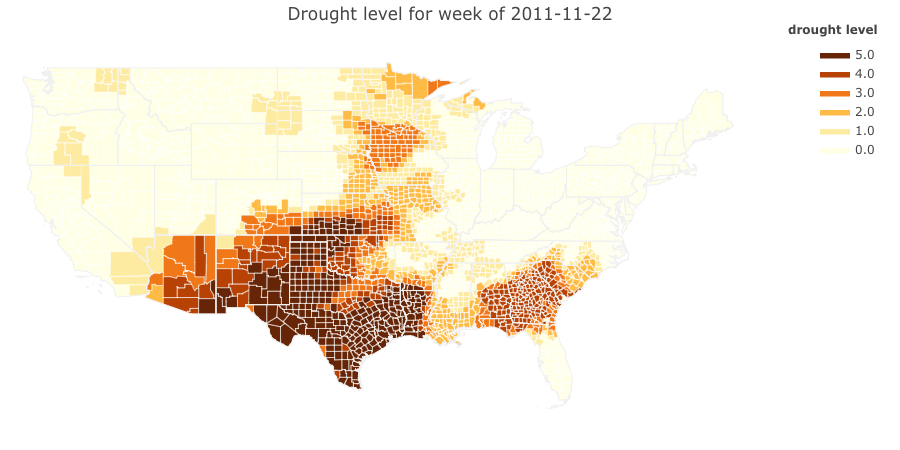
\includegraphics[width =  \textwidth]{DroughtLevel_wk_2011-11-22.png}
    \caption{Drought map of the Continental United States during the week of November 22\textsuperscript{nd}, 2011.}
    \label{fig:fullmap1}
\end{figure}

\begin{figure}[hbt!]
    \centering
    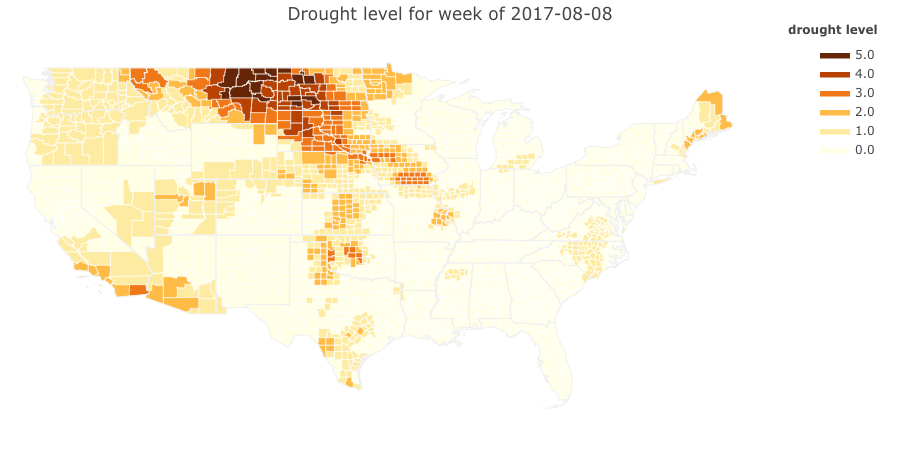
\includegraphics[width =  \textwidth]{DroughtLevel_wk_2017-08-08.png}
    \caption{Drought map of the Continental United States during the week of August 8\textsuperscript{th}, 2017.}
    \label{fig:fullmap2}
\end{figure}


\clearpage 
\subsection{Spacial prediction of county drought level}

The hyperparameter of our KAN model is degree of separation, which controls the number of surrounding neighbors that are eligible to vote for a particular county. In order to optimize our model, we performed 8-fold cross validation, finding the degree of separation that maximized the accuracy of prediction. Here, our metric for determining accuracy is mean squared error. Our 8-fold cross validation set consists of drought data of all U.S. counties taken at eight random time points between 2010 and 2017. 

\begin{figure}[hbt!]
    \centering
    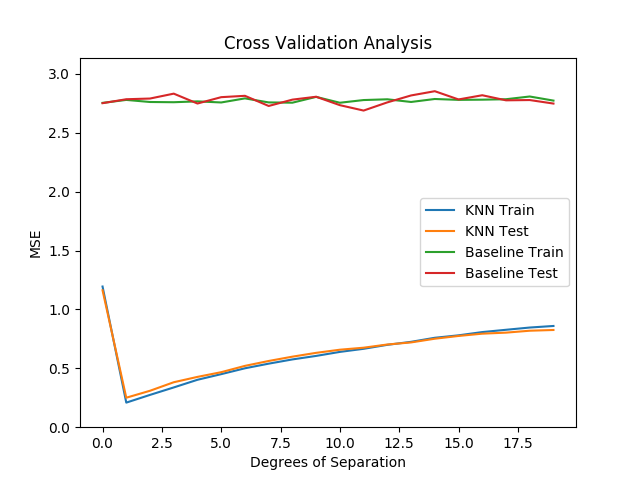
\includegraphics[width = 0.8 \textwidth]{CV_knn.png}
    \caption{Cross validation results for the KAN.}
    \label{fig:CV}
\end{figure}

Our cross validation results show that the  optimal degree of separation is one, yielding a mean squared error of 0.25 (Fig. \ref{fig:CV}). For reference, the baseline classifier consistently yields a mean squared error of 2.75. Our findings indicate that for any given county, the counties that are directly adjacent to it offers the best drought prediction.

For our held-out test set, we selected drought data during the week of December 12\textsuperscript{th}, 2017. 

We randomly selected 20\% of all the counties in United States to hold out as our test set. Then, using our best KAN model determined from 
cross validation, we trained our model on the other 80\% of the counties. With this test set, our model yielded a mean square error of 0.20, as expected from our cross validation results. 
Classification results of our testing set are shown in Figures \ref{fig:training}, \ref{fig:ground_truth}, \ref{fig:predicted}, \ref{fig:full_ground_truth}, and  \ref{fig:full_predicted}.


\begin{figure}[hbt!]
    \centering
    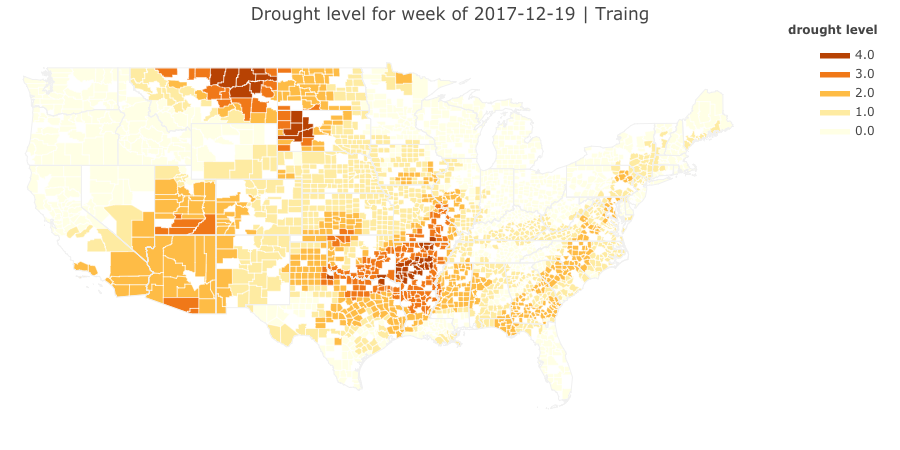
\includegraphics[width =  \textwidth]{training.png}
    \caption{80\% of counties used for training our KAN}
    \label{fig:training}
\end{figure}


\begin{figure}[hbt!]
    \centering
    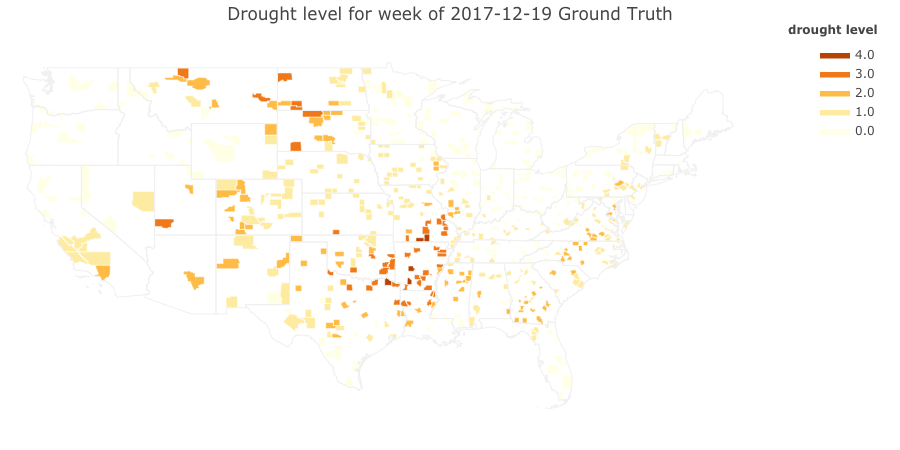
\includegraphics[width =  \textwidth]{ground_truth.png}
    \caption{Ground truth for the 20\% of the counties used for testing.}
    \label{fig:ground_truth}
\end{figure}


\begin{figure}[hbt!]
    \centering
    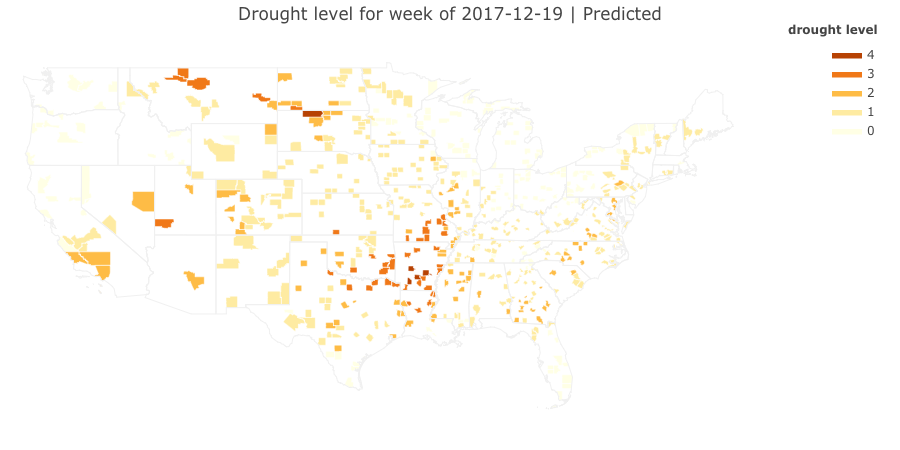
\includegraphics[width =  \textwidth]{predicted.png}
    \caption{Predicted drought levels for the 20\% of counties used for testing.}
    \label{fig:predicted}
\end{figure}



\begin{figure}[hbt!]
    \centering
    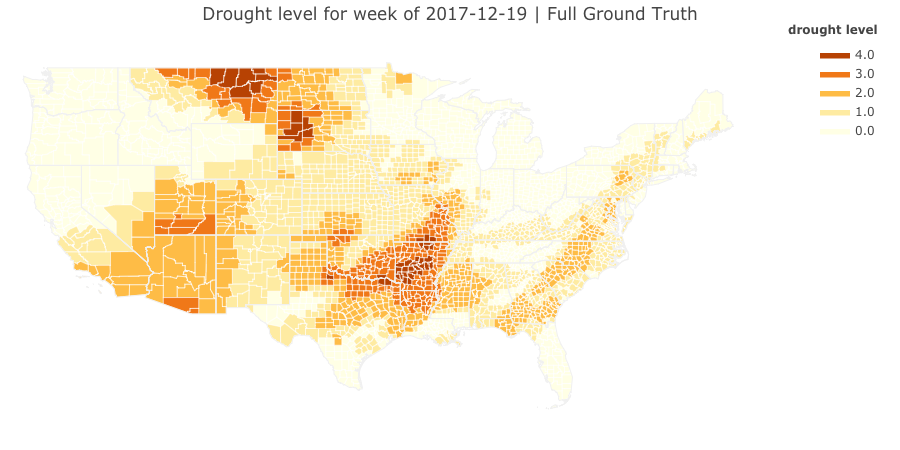
\includegraphics[width =  \textwidth]{full_ground_truth.png}
    \caption{Full map of the original drought data on December 12th, 2017. }
    \label{fig:full_ground_truth}
\end{figure}


\begin{figure}[hbt!]
    \centering
    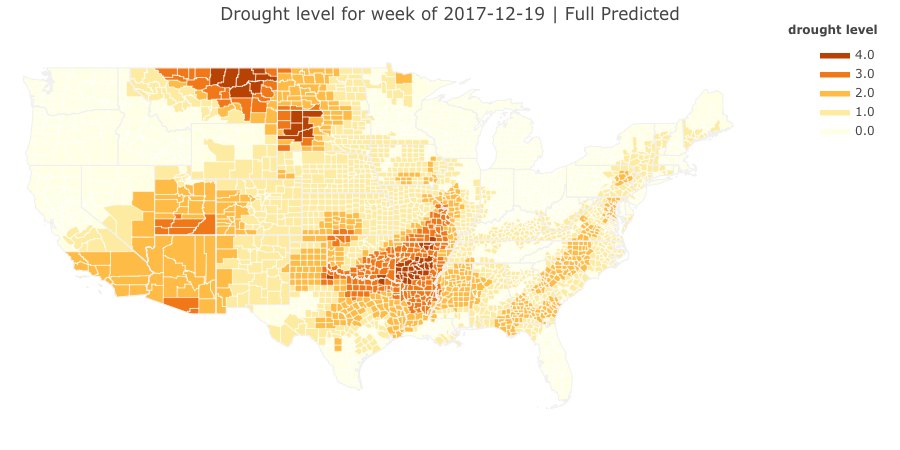
\includegraphics[width =  \textwidth]{full_predicted.png}
    \caption{Full map of the predicted drought data on December 12th, 2017.}
    \label{fig:full_predicted}
\end{figure}

\clearpage
\subsection{Spacial and temporal identification of Dissimilar Drought Counties}

We have identified a total of 45 groups of Dissimilar Drought Counties (DDC) based on their pairwise Dynamic Time Warping distances. Figure \ref{fig:maxdist_grp10} shows an example of a DDC where, years 2015 and 2016 saw a large and extended disparity in drought levels among Orange County, CA (level 4); San Bernardino County, CA (level 3); Imperial County, CA (level 2); and La Paz County, AZ (level 1). A map visualization of the drought levels for this set of DDC is displayed in Figure \ref{fig:grp10}. 

\begin{figure}[hbt!]
    \centering
    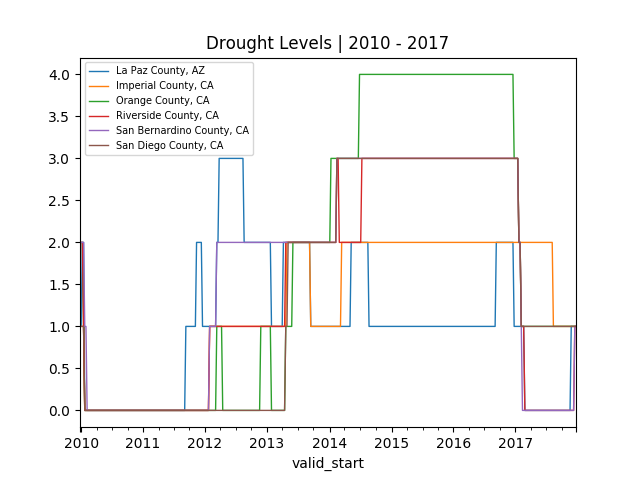
\includegraphics[width = 0.8 \textwidth]{max_dist_group10.png}
    \caption{Plot of drought levels over time for a group of DDC.}
    \label{fig:maxdist_grp10}
\end{figure}

\begin{figure}[hbt!]
    \centering
    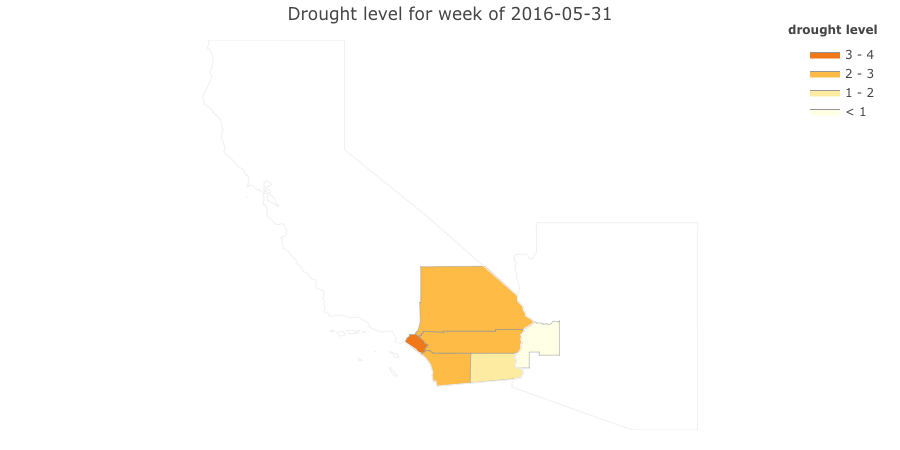
\includegraphics[width = \textwidth]{DroughtLevel_group10__wk_2016-05-31.png}
    \caption{May 5th, 2016 drought map of 
    La Paz County, AZ; 
    Imperial County, CA;
    Orange County, CA;
    Riverside County, CA; San Bernardino County, CA; and San Diego County, CA. }
    \label{fig:grp10}
\end{figure}

A second example of a DDC is shown in Figures \ref{fig:maxdist_grp16} and \ref{fig:grp16}. 

\begin{figure}[hbt!]
    \centering
    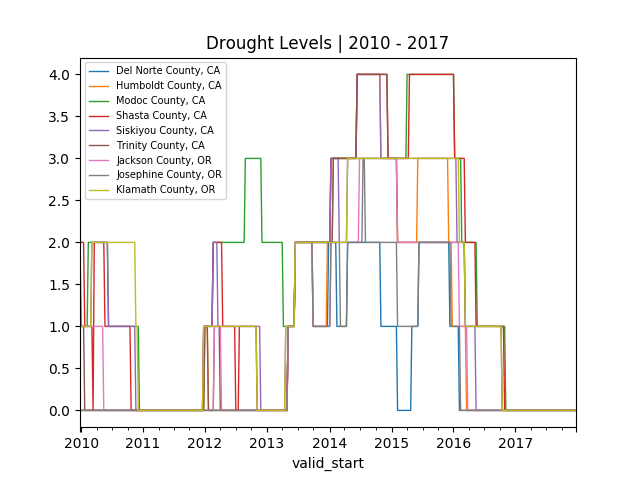
\includegraphics[width = 0.8 \textwidth]{max_dist_group16.png}
    \caption{Plot of drought levels over time for a group of DDC.}
    \label{fig:maxdist_grp16}
\end{figure}


\begin{figure}[hbt!]
    \centering
    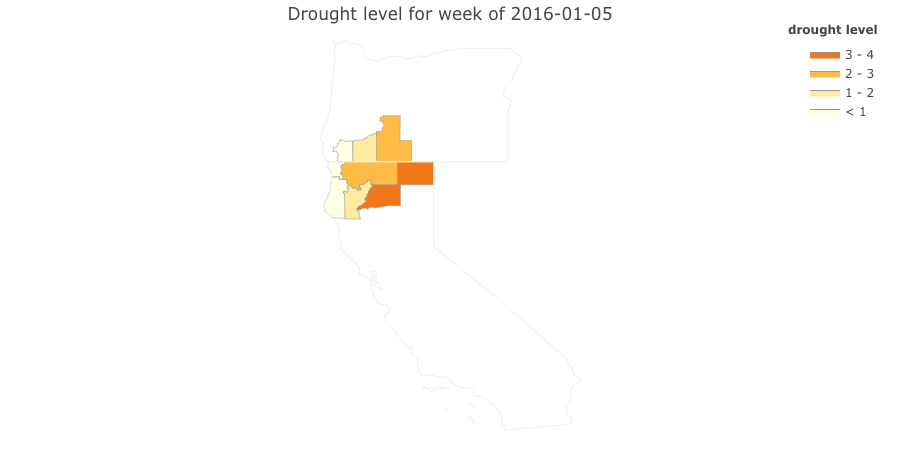
\includegraphics[width = \textwidth]{DroughtLevel_group16__wk_2016-01-05.png}
    \caption{January 1st, 2016 drought map of 
    Del Norte County, CA; 
    Humboldt County, CA;
    Modoc County, CA;
    Shasta County, CA;
    Siskiyou County, CA;
    Trinity County, CA;
    Jackson County, OR;
    Josephine County, OR;
    Klamath County, OR.}
    \label{fig:grp16}
\end{figure}

For comparison, a groups of adjacent counties that have very low Dynamic Time Warping distances experience very similar trends in drought levels, and thus are not viable candidates for water resource reallocation (Fig. \ref{fig:min_dist_group07}). 

\begin{figure}[hbt!]
    \centering
    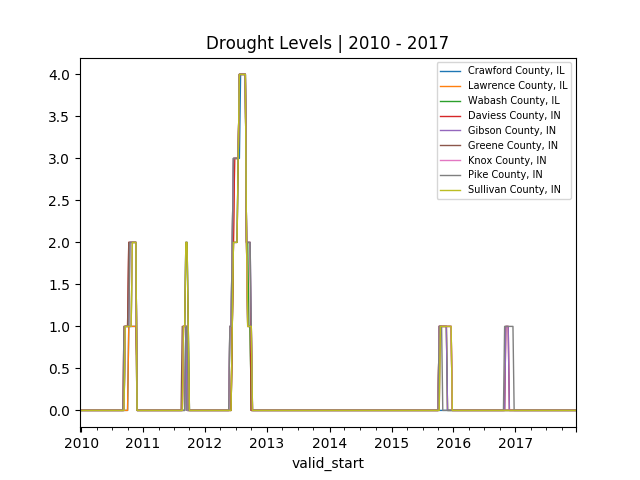
\includegraphics[width = 0.8 \textwidth]{min_dist_group07.png}
    \caption{}
    \label{fig:min_dist_group07}
\end{figure}

\clearpage

\section{Conclusion}
Using statistical methods and machine learning approaches, this paper analyzes the patterns of drought levels in the United States and how they might reveal possible suggestions to mitigate the effects of drought. More specifically, we sought to answer the following question: For a specified county at a given time, can we determine its drought level based on the drought levels of its neighboring counties?

Our KAN classifier revealed that, for any given county, the counties directly adjacent to it offer the best data to determine the most accurate drought level. Furthermore, our KAN classifier performed significantly better than the baseline classifier. In fact, evaluating our model on a held-out test set resulted in a mean square error of 0.20, which is approximately 92\% more accurate than our baseline.

It is important to note that our KAN classifier assumes that counties near each other have similar drought levels. However, after analyzing the distribution of drought levels throughout the U.S., we found that it is not necessarily true that all neighboring counties have similar drought levels. This led us to investigate whether we could answer a new question: Can we identify Dissimilar Drought Counties (DDC)?


Our algorithm, which exploits the time series distance metric Dynamic Time Warping, effectively 
identified 45 groups of DDC. With these results, we can suggest ways to to be help local water companies make informed and drought-conscious decisions for reallocating water to various counties within its domain. For example, consider the Golden State Water Company, which serves counties in California such as Imperial County, Orange County, San Bernardino County, as well as others.\cite{Companies:2019} The results from our algorithm show that some of these counties were identified in a DDC group, which is seen in Figure \ref{fig:grp10}. Consequently, the Golden State Water Company can reallocate its water supply such that it distributes more water to the counties that experience a higher severity of drought while cutting back water supply in counties that are not experiencing as severe of a drought. Thus, our algorithm, if incorporated into the management of water companies, may temporarily help alleviate the negative effects of drought.


\clearpage
%--------------------
%	BIBLIOGRAPHY
%--------------------

\bibliographystyle{unsrt}

\bibliography{WorksCited}

%--------------------------

\end{document}